\section{Neutron Efficiency}
\par
For calculating the neutron efficiency during SR1 calibrations, AmLi was used.
As seen in \autoref{sec:sec:od_simulation_efficiency}, the efficiency is no longer expected to meet the requirement of 95\% efficiency.
But, as has been shown in the previous section, the simulation significantly underestimates the light collection efficiency, and so it's possible that the neutron propagation is also not modelled adequately.

\par
Three AmLi sources were used at the same time during this calibration, each placed in a different CSD tube.
This is summarised in \autoref{tab:amli_source_activities}.

\begin{table}[!htbp]
    \centering
    \begin{tabular}{c|c|c}
        CSD & AmLi Source No. & Activity (n/s) \\ \hline
        1   & Source-2        & 13.8           \\
        2   & Source-1        & 9.3            \\ 
        3   & Source-3        & 11.9                
    \end{tabular}
    \caption{AmLi source activities in each CSD}
    \label{tab:amli_source_activities}
\end{table}

\par
For this data, the S2-trigger was used, and the cuts developed for the WIMP search were used to filter out unusable data, to leave a fairly pure dataset of neutron recoils.
These are summarised below, but are detailed in \cite{lz_ws_sr1_ref};

\begin{enumerate}
    \item \textbf{SS}: Single Scatter cut as determined by the interaction finder, shown to be 98.5\% efficient.
    \item \textbf{S2Cuts}: Remove events where the S2 pulse has unusual properties.
    \item \textbf{S1Cuts}: Remove events where the S1 pulse has unusual properties.
    \item \textbf{FID}: Fiducial Volume, to remove wall events and ensure that the neutron penetrated deep enough.
    \item \textbf{NR}: Select events that have nuclear recoiled by selecting events within 1-$\sigma$ of the NR band, which was calibrated using the external DD neutron source.
\end{enumerate}

\par
Three positions in the CSD were used, 0mm, 700mm and 1400mm. 
These definitions are identical to those used in \autoref{sec:od_simulation_efficiency}.
The result of applying the selection cuts to these runs is shown in \autoref{tab:amli_calibration_summary}.

\begin{table}[!htbp]
    \centering
    \begin{tabular}{c|c|c|c|c}
        \multirow{2}{*}{z position (mm)} & \multirow{2}{*}{Run IDs}  & \multicolumn3{c}{Number}  \\ 
                                         &                           & Events    & SS & passing all cuts     \\ \hline
        0                                & 8350-8369                 & 5,504,700 & X  & X               \\
        700                              & 8304-8317                 & 3,688,200 & X  & X               \\ 
        1400                             & 8319-8348                 & 7,041,500 & X  & X                
    \end{tabular}
    \caption{Summary of AmLi source deployment during post SR1 calibrations}
    \label{tab:amli_calibration_summary}
\end{table}

\par
From these events it is then possible to search for events that occur after the S1 in both the Skin and OD.
Those events which pass the TPC cuts are shown in XXX.




\par
Using the maximum veto window for 200keV of 1200$\mu$s, the efficiency as a function of photons detected is shown in \autoref{fig:commissioning_amli_efficiency_per_phd}.
The combined veto efficiency of the Skin and OD are used here due to the limited impact the Skin has on the veto efficiency of neutrons.

\begin{figure}[!htbp]%
\centering
\begin{tikzpicture}
\centering
    \begin{axis}[
            ylabel=Efficiency (\%),
            xlabel=Photons Detected (phd),
            width=15cm,
            height=8cm,
            grid=major,
            xmin=0, xmax=100,
            %ymin=45, ymax=100,
            %minor y tick num=1,
            ]
        \addplot[red,
                 error bars/.cd, error bar style={color=red},
                 y dir=both, y explicit, 
                 x dir=both, x explicit,
                 ]
            table [x=bin,y=value, y error minus index=4, y error plus index=5, x error minus index=2, x error plus index=3,]
            {Data/Neutron_Efficiency/AmLi_Commissioning/pos_0_efficiency_per_phd.dat};    
        \addplot[green, 
                 error bars/.cd, error bar style={color=green},
                 y dir=both, y explicit, 
                 x dir=both, x explicit,
                 ]
            table [x=bin,y=value, y error minus index=4, y error plus index=5, x error minus index=2, x error plus index=3,]
            {Data/Neutron_Efficiency/AmLi_Commissioning/pos_700_efficiency_per_phd.dat};             
        \addplot[blue,
                 error bars/.cd, error bar style={color=blue},
                 y dir=both, y explicit, 
                 x dir=both, x explicit,
                 ]
            table [x=bin,y=value, y error minus index=4, y error plus index=5, x error minus index=2, x error plus index=3,]
            {Data/Neutron_Efficiency/AmLi_Commissioning/pos_1400_efficiency_per_phd.dat};    
        \legend{0mm,700mm,1400mm}  
            
    \end{axis}
            
\end{tikzpicture}
    \caption{Efficiency as a function of pulse area}
    \label{fig:commissioning_amli_efficiency_per_phd}
\end{figure}


\par
Due to the poorer than expected performance of the OD for tagging neutrons, the decision was made to use the longer veto window of 1200$\mu$ combined with a 200keV pulse requirement in the OD or a 100keV requirement in the Skin.
The result of this is summarised in \autoref{fig:commissioning_amli_efficiency_with_bg_rate}.

\begin{figure}[]%
\centering
\begin{tikzpicture}
\centering
    \begin{axis}[
            ylabel=Efficiency (\%),
            xlabel=Time ($\mu$s),
            width=14cm,
            height=8cm,
            grid=major,
            axis y line*=left,
            xmin=0, xmax=1500,
            ymin=45, ymax=100,
            minor y tick num=1,
            legend style = { column sep = 10pt, legend columns = -1,},
            legend pos=north west,
            ]
        \addplot+[red, mark=none, forget plot]
                  table [x=bin,y=value]
                  {Data/Neutron_Efficiency/AmLi_Commissioning/pos_0_od_200kev_efficiency.dat};   
        \addplot[red, only marks, mark size=1.0pt,
                 error bar legend,
                 error bars/.cd, error bar style={color=black},
                 y dir=both, y explicit, 
                 x dir=both, x explicit,
                 ]
            table [x=bin,y=value, y error minus index=4, y error plus index=5, x error minus index=2, x error plus index=3,]
            {Data/Neutron_Efficiency/AmLi_Commissioning/pos_0_od_200kev_efficiency.dat};    
            
        \addplot+[green, mark=none, forget plot]
          table [x=bin,y=value]
          {Data/Neutron_Efficiency/AmLi_Commissioning/pos_700_od_200kev_efficiency.dat};      
        \addplot[green, 
                 only marks, mark size=1.0pt,
                 error bar legend,
                 error bars/.cd, error bar style={color=black},
                 y dir=both, y explicit, 
                 x dir=both, x explicit,
                 ]
            table [x=bin,y=value, y error minus index=4, y error plus index=5, x error minus index=2, x error plus index=3,]
            {Data/Neutron_Efficiency/AmLi_Commissioning/pos_700_od_200kev_efficiency.dat};       
            
        \addplot+[blue, mark=none, forget plot]
          table [x=bin,y=value]
          {Data/Neutron_Efficiency/AmLi_Commissioning/pos_1400_od_200kev_efficiency.dat};         
        \addplot[blue, 
                 only marks, mark size=1.0pt,
                 error bar legend,
                 error bars/.cd, error bar style={color=black},
                 y dir=both, y explicit, 
                 x dir=both, x explicit,
                 ]
            table [x=bin,y=value, y error minus index=4, y error plus index=5, x error minus index=2, x error plus index=3,]
            {Data/Neutron_Efficiency/AmLi_Commissioning/pos_1400_od_200kev_efficiency.dat};    
        \legend{0mm,700mm,1400mm}  
            
    \end{axis}
    \begin{axis}[
            ylabel=False Veto (\%),
            yticklabel pos=right,
            axis y line*=right,
            axis x line=none,
            width=14cm,
            height=8cm,
            %grid=major,
            xmin=0, xmax=1500,
            ymin=0, ymax=50,
            minor y tick num=9,]
        \addplot[domain=0:1500,
            samples=3,
            ]
            {x * 42.5 * 100 / 1000000};
        \iffalse
        \addplot[domain=0:1500,
            samples=3,
            ]
            {x * 95.8 * 100 / 1000000};        
        \addplot[domain=0:1500,
            samples=3,
            ]
            {x * 276.8 * 100 / 1000000};  
        \fi
         \addplot[dashed, mark=none, red] coordinates {(0,5) (1500,5)};
         
        % \node[rotate=24] at (axis cs: 1000,26) {276.8Hz};
        % \node[rotate=11] at (axis cs: 1400,15.5) {95.8Hz};
         \node[rotate=5] at (axis cs: 1400,8) {42.5Hz};
    \end{axis}
            
\end{tikzpicture}
    \caption{Neutron tagging efficiency from AmLi at each height for the 200~keV phe threshold.
    The horizontal dashed line is the 5\% impact on live-time requirement.
    The black line is the 200~keV background rate in the OD.}
    \label{fig:commissioning_amli_efficiency_with_bg_rate}
\end{figure}


\par
On SR1 WIMP-search data, this has a total impact of 4.99\% on live-time, and the resultant events which were vetoed are shown in Figure XXX.
No neutrons were vetoed in SR1 which corresponds to no neutrons being expected.
The events which were vetoed were electron recoil events which were coincidence with an OD background.

\begin{figure}[!htbp]
    \centering
    
\includegraphics[width=0.5\textwidth]{Figures/Placeholder.png}
    \caption{Effect on SR1 data before and after the \textbf{Veto} cut.}
    \label{fig:tpc_with_od_veto_in_sr1}
\end{figure}

\par
The AmLi 

\begin{figure}[]%
\centering
\begin{tikzpicture}
\centering
    \begin{axis}[
            ylabel=Log10(S2) (phd),
            xlabel=S1 (phd),
            width=15cm,
            height=8cm,
            xmin=0, xmax=600,
            ymin=3, ymax=5,
            %ymin=45, ymax=100,
            %minor y tick num=1,
            ]
            
        \addplot[black, only marks, mark=+]
            table []
            {Data/Neutron_Efficiency/AmLi_Commissioning/s1s2_passed_od_veto_in_fid.dat};    
        \addplot[green, only marks, mark=o]
            table []
            {Data/Neutron_Efficiency/AmLi_Commissioning/s1s2_failed_od_veto_in_fid.dat};
        
        \addplot[blue, ]
            table [x=s1c, y=mean]
            {Data/tpc/sr1_er_band.dat};     
        \addplot[blue, dashed]
            table [x=s1c, y=nsig1]
            {Data/tpc/sr1_er_band.dat};     
        \addplot[blue, dashed]
            table [x=s1c, y=psig1]
            {Data/tpc/sr1_er_band.dat};     

        \addplot[red, ]
            table [x=s1c, y=mean]
            {Data/tpc/sr1_nr_band.dat};     
        \addplot[red, dashed]
            table [x=s1c, y=nsig1]
            {Data/tpc/sr1_nr_band.dat};     
        \addplot[red, dashed]
            table [x=s1c, y=psig1]
            {Data/tpc/sr1_nr_band.dat};     
            
    \end{axis}
            
\end{tikzpicture}
    \caption{TPC events vetoed by the OD. In Red are events which passed all cuts including the OD veto. In Blue are events which passed all cuts except the OD veto.}
    \label{fig:sr1_vetoed_events}
\end{figure}


\subsection{Neutron Captures}
\par
Although AmLi 
Another source that can be used to study the neutron capture time is the ${}^{252}{Cf}$ calibration source.
Spontaneous fission of ${}^{252}{Cf}$ typically results in a number of $\gamma$'s with a combined energy of up to 10MeV which are accompanied by a number of neutrons.
An example event from the LZ calibration run pre-SR1 is shown in \autoref{fig:cf252_event_viewer}.
This allows for neutrons to be tagged by tagging the fission by coincident $\gamma$'s in a each detector, and assuming later pulses are dominated by neutrons.

\begin{figure}[!htbp]
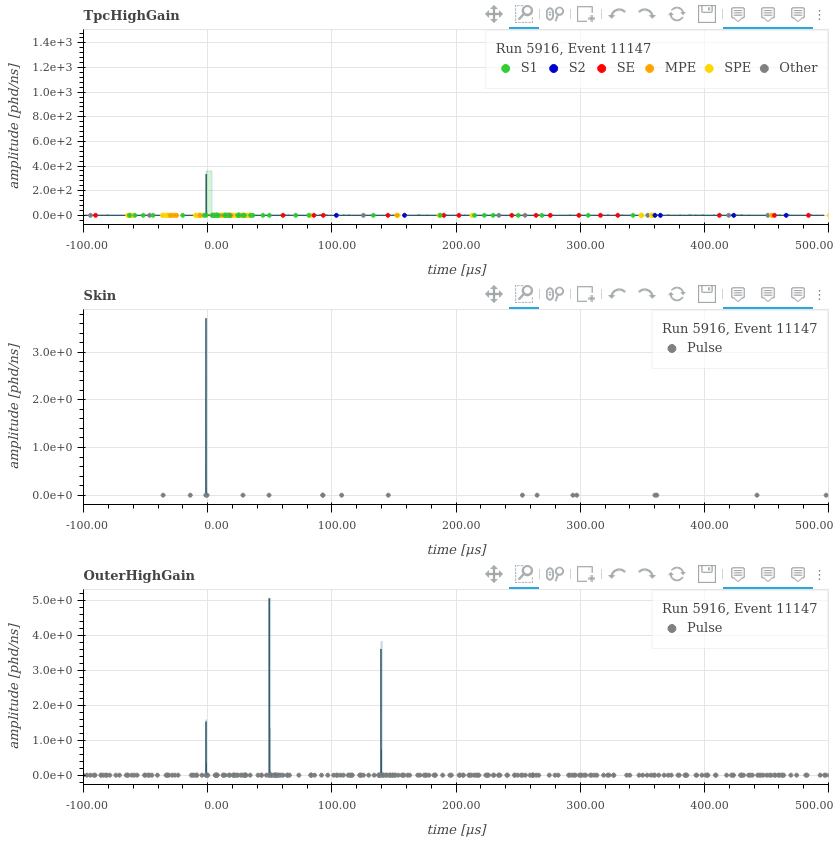
\includegraphics[width=\textwidth]{Figures/NeutronCaptureTime/cf252_eventviewer_5916.png}
\centering
\caption{Example event from ${}^{252}{Cf}$ calibration run showing the $\gamma$'s causing coincident pulses in each detector followed by two neutrons being captured in the Outer Detector}
\label{fig:cf252_event_viewer}
\end{figure}

\par
Although \autoref{fig:cf252_event_viewer} indicates that prompt $\gamma$'s can be used for tagging it does come with a significant caveat; namely that expressed in \autoref{fig:fission_fragments_time}.
There is a non-insignificant probability that $\gamma$'s will be emitted at the same time as a $\gamma$ from a neutron capture is released.
Additionally the majority of study into prompt $\gamma$'s from fission focus on the first 100ns post-fission and the energy and multiplicity beyond that time is not well theorised. 
However, by selecting events which only have a double or triple detector coincidence this can be mitigated.


\begin{figure}[!htbp]
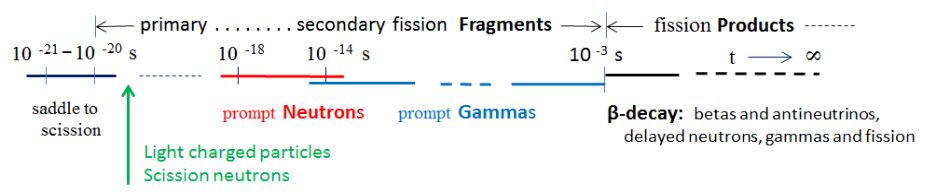
\includegraphics[width=13cm]{Figures/NeutronCaptureTime/fission_fragment_times.png}
\centering
\caption{Emission time-frame of fission components. Adapted from \cite{cf252_fission_ref}}
\label{fig:fission_fragments_time}
\end{figure}

\begin{figure}[]%
\centering
\begin{tikzpicture}
\centering
    \begin{axis}[
            ylabel=Count,
            xlabel=Pulse Area (phd),
            width=15cm,
            height=8cm,
            grid=major,
            xmin=0, xmax=2500,
            ymode=log,
            %ymin=45, ymax=100,
            %minor y tick num=1,
            ]
        \addplot[red, only marks, mark size=1.0,
                 error bar legend,
                 error bars/.cd, error bar style={color=black},
                 y dir=both, y explicit, 
                 x dir=both, x explicit,
                 ]
            table [x=pulsearea,y=weight, x error=xerror, y error=yerror]
            {Data/cf252/cf252_od_pulses_before400ns.dat};    
        \addplot[green, only marks, mark size=1.0,
                 error bar legend,
                 error bars/.cd, error bar style={color=black},
                 y dir=both, y explicit, 
                 x dir=both, x explicit,
                 ]
            table [x=pulsearea,y=weight, x error=xerror, y error=yerror]
            {Data/cf252/cf252_od_pulses_within400ns.dat};           
        \addplot[blue, only marks, mark size=1.0,
                 error bar legend,
                 error bars/.cd, error bar style={color=black},
                 y dir=both, y explicit, 
                 x dir=both, x explicit,
                 ]
            table [x=pulsearea,y=weight, x error=xerror, y error=yerror]
            {Data/cf252/cf252_od_pulses_after400ns.dat};
        \legend{Before 400ns,Within 400ns,After 400ns}  
            
    \end{axis}
            
\end{tikzpicture}
    \caption{Pulse Distribution depending upon when the tagging pulse was.}
    \label{fig:cf252_pulse_selection}
\end{figure}

\begin{figure}[!htbp]%
\centering
\begin{tikzpicture}
\centering
    \begin{axis}[
            ylabel=Count,
            xlabel=Photons Detected (phd),
            width=15cm,
            height=8cm,
            grid=major,
            xmin=0, xmax=2500,
            %ymin=45, ymax=100,
            %minor y tick num=1,
            ]
        \addplot[black, only marks, mark size=1.0,
                 error bars/.cd, error bar style={color=black},
                 y dir=both, y explicit, 
                 x dir=both, x explicit,
                 ]
            table [x=pulsearea,y=weight, x error=xerror, y error=yerror]
            {Data/cf252/cf252_od_largest_after400ns.dat}; 
            
    \end{axis}
            
\end{tikzpicture}
    \caption{Largest OD pulse in an event window 400ns after the first coincidence pulse.}
    \label{fig:cf252_gd152_captures}
\end{figure}

\begin{figure}[]%
\centering
\begin{tikzpicture}
\centering
    \begin{axis}[
            ylabel=Count,
            xlabel=Capture Time ($\mu$s),
            width=15cm,
            height=8cm,
            grid=major,
            ymode=log,
            xmin=-10,xmax=1000,
            ymin=1,
            %minor y tick num=1,
            ]
        \addplot[black, only marks, mark size=0.5,
                 error bars/.cd, error bar style={color=black},
                 y dir=both, y explicit, 
                 x dir=both, x explicit,
                 ]
            table [x=time,y=weight, x error=xerror, y error=yerror]
            {Data/cf252/cf252_gd_capture_time.dat}; 
            
        \addplot[red,
                 domain=15:1500,
                 ]
            {2305 * exp(-x/30.5) + 342 * exp(-x/125.2) + 0.9663}; 
            
        \addplot[blue,
                 domain=15:1500,
                 ]
            {2294 * exp(-x/31.2) + 235 * exp(-x/70.1) + 11.94 * exp(-x/176.4)}; 
            
    \end{axis}
            
\end{tikzpicture}
    \caption{Pulse Distribution depending upon when the tagging pulse was.
             In red is the best fit from 2 exponential decays.
             In blue is the expected neutron capture time.}
    \label{fig:cf252_gd_capture_time}
\end{figure}

\par
The best fit was found to be with just two exponents.
With $t_0 = 31.39 \pm 0.4\mu s$ and $t_1 = 124.5 \pm 1.7\mu s$, with a $\chi^2=0.821$.
$t_0$ accounts for neutrons which travel straight through from the source position to the GdLS and are captured on the GdLS.
$t_1$ is more complex as it accounts for neutrons scatter several times in not the GdLS, such as the acrylic of foam regions.
Given each of these have a different affect on this, it is not clear exactly what is causing it.
This is particularly apparent when compared to the expected result from simulations (also included in \autoref{fig:cf252_gd_capture_time}, where we can see that the neutrons are taking longer than expected to be captured in the OD.
This indicates that neutrons are becoming trapped in materials between the calibration tube and the OD.
The possible materials between the CSD and the OD are primarily foam, acrylic and water.
Given that the acrylic thickness was measured during construction, this leaves water as the most likely scenario.

\par
One possible reason for this is the foam surrounding the OCV not stopping all water from coming into that region.
Though when the SATs were installed, there was no discernible gap between the SAT and the Tyvek around the OCV foam.
Though it is possible that a small amount of water would have entered this area over time, but no more than a few mm.

\par
Another possibility is that the foam became at least in part filled with water.
Water ingress in foam has been well studied at least in part, with the industrial measures of water absorption defined as via diffusion and by submersion \cite{foam_with_water_ref}.
The effectiveness of any foam type to keep water out is based on a number of factors including density and most importantly if the structure is closed or open\footnote{in terms of whether the cells which make up the foam structure. Open cell foams are softer and more flexible as each cell is open to the atmosphere. Closed cell foams are firmer with the majority of cells being closed to the atmosphere.}.
The difference in terms of water ingress is shown in \autoref{fig:foam_mri_water_ingress}.


\begin{figure}[!tbhp]
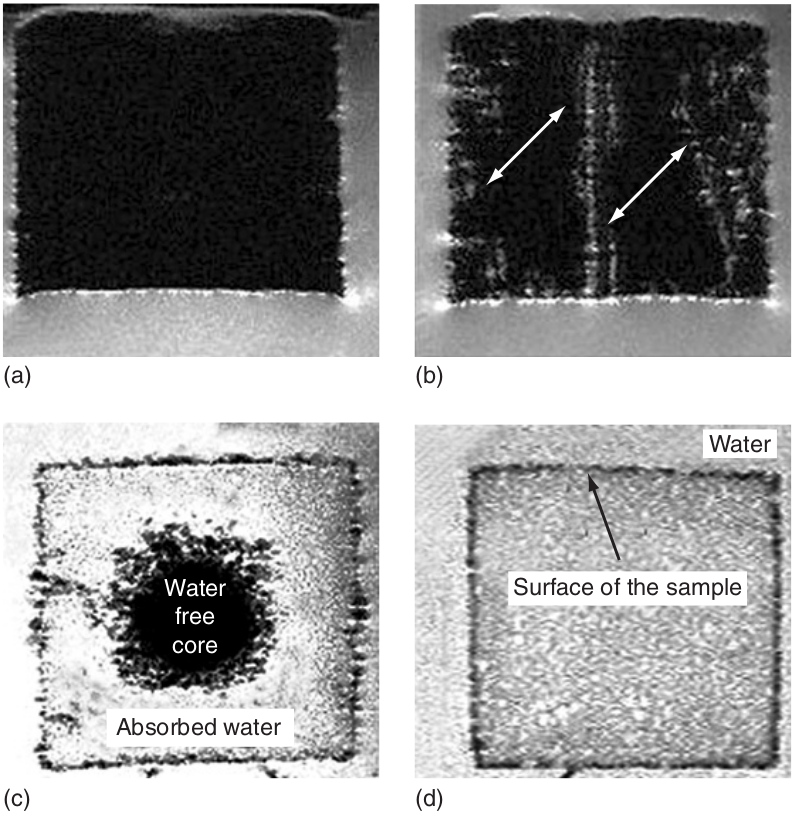
\includegraphics[width=\textwidth]{Figures/NeutronCaptureTime/foam_water_absorption.png}
\centering
\caption{Magnetic resonance images of 30 mm cube samples of polyurethane foam for two types of different foam of the same density, 0.3 g m${}^{-3}$: a closed cell foam (top) and an open cell foam (bottom).
(a) closed cell foam after 8 hours. (b) closed cell foam after 63 hours.
(c) open cell foam after 8 hours. (d) open cell foam after 72 hours.
Images from \cite{foam_mri_data_ref}.
}
\label{fig:foam_mri_water_ingress}
\end{figure}


\par
The foam installed around the OCV (green foam in \autoref{sec:od_construction_sec}) is a closed cell foam expanded using $CO_2$, so each cell is filled with $CO_2$, foam 3000 CS in \cite{styrodur_water_ingress_ref}.
As such the foam is expected to experience a 0.7\% volume ingress of water due to long term submersion and 5\% volume ingress of water from diffusion\footnote{long-term in this case refers to a 28-day test as is the industry standard, see BS EN ISO 16535 (BS EN 12087) and BS EN ISO 16536 (previously BS EN 12088).}.
These values, being based off of tests designed of industry do not necessarily map obviously onto how it was used in this application, particularly given that water pressure is not considered in the industrial tests and the long-term are orders of magnitude less than the exposure the LZ foam has had already.
\par
In order to begin probing this, a test was conducted to observe what happens to this foam (and what happens to the water).
An example of each piece of foam used, was placed in de-ionised water and placed under a $N_2$ purge. 
The water resistivity was measured every few hours as a monitor of the water's purity.
The result over the first week of running is shown in \autoref{fig:od_foam_degredation}.
What is observed during this period is the water becoming contaminated with ions from the foam from out gassing.
Over a longer period of study it may show that the foam becomes saturated with water, particularly with a test using a piece of foam shaped to the same dimensions as those used in the installation.

\par
In relation to LZ, this has two impacts, firstly these ions can circulate throughout the OD water and contribute to the low energy rate.
Secondly, this will impact on the time it takes for a neutron to reach the GdLS.
Taking the most extreme case as the foam being completely replaced with water, we can see that the neutron time to reach the GdLS is significantly increased (shown in blue in \autoref{fig:data_vs_sim_gd_capture_time}).
This therefore seems an reasonable explanation for the difference observed.

\begin{figure}[]%
\centering
\begin{tikzpicture}
\centering
    \begin{axis}[
            xlabel=Time (hours),
            ylabel=Resistivity (mS/cm),
            width=15cm,
            height=8cm,
            grid=major,
            xmin=-1, xmax=250,
            legend style={at={(0.95,0.5)},anchor=east},
            %ymin=45, ymax=100,
            %minor y tick num=1,
            ]
        \addplot[green, only marks,
                 error bars/.cd, error bar style={color=black},
                 y dir=both, y explicit, 
                 ]
            table [x=time,y=di,y error=error]
            {Data/cf252/foam_in_di_water.dat}; 
        \addplot[blue, only marks,
                 error bars/.cd, error bar style={color=black},
                 y dir=both, y explicit, 
                 ]
            table [x=time,y=foam,y error=error]
            {Data/cf252/foam_in_di_water.dat}; 
        \addplot[red, dashed,
                 domain=-10:750,
                 samples=3]
                {1};
            
        \legend{Control, Foam,};
    \end{axis}
            
\end{tikzpicture}
    \caption{Measure of water purity from foam used in the OCV.
             Both the Control (just water) and the Foam (water with foam pieces) were under $N_2$ purge for the duration of the data taking.
             The dashed red line indicated the Type 2 DI water limit.}
    \label{fig:od_foam_degredation}
\end{figure}

\begin{figure}[]%
\centering
\begin{tikzpicture}
\centering
    \begin{axis}[
            ylabel=Count (Arb.),
            xlabel=Capture Time ($\mu$s),
            width=15cm,
            height=8cm,
            grid=major,
            ymode=log,
            xmin=-10,xmax=800,
            ymin=1e-3, ymax=5,
            %minor y tick num=1,
            ]
        \addplot[black, only marks, mark size=0.5,
                 error bars/.cd, error bar style={color=black},
                 y dir=both, y explicit, 
                 ]
            table [x=time,y=weight, y error=yerror]
            {Data/cf252/cf252_gd_capture_time_normed.dat}; 
            
        \addplot[red, const plot]
            table [x=time,y=weight]
            {Data/cf252/amli_0mm_default.dat}; 
            
        \addplot[green, const plot]
            table [x=time,y=weight]
            {Data/cf252/amli_0mm_water_saturated.dat}; 

        \addplot[blue, const plot]
            table [x=time,y=weight]
            {Data/cf252/amli_0mm_water.dat}; 
            
    \end{axis}
            
\end{tikzpicture}
    \caption{Neutron capture time on Gadolinium in the OD. The observed capture time from ${}^{252}$Cf is shown in black. In red is the expected capture time from simulation. In green is the capture time if the foam has been saturated with water up to 5\% of its volume. In blue is the capture time if all foam around the OCV has been replaced with water. Each distribution has been normalised the maximum value.}
    \label{fig:data_vs_sim_gd_capture_time}
\end{figure}
